103. \begin{figure}[ht!]
\center{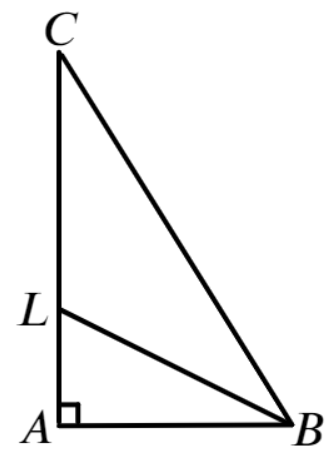
\includegraphics[scale=0.35]{g9-103.png}}
\end{figure}\\
По теореме Пифагора имеем $AC=\sqrt{576-9}=9\sqrt{7}$см. По свойству основания биссектрисы получаем соотношение $\cfrac{AL}{LC}=\cfrac{AB}{BC}=\cfrac{3}{24}=\cfrac{1}{8},$ значит $AL=\cfrac{1}{9}\cdot9\sqrt{7}=\sqrt{7}$см. Тогда  по теореме Пифагора $BL=\sqrt{7+9}=4$см.\\
